\section{SOI}
\subsection{Introduction}
\subsection{Recent Milestones}
At present, major issues in the SOI pixel development are ``back-gate effect'', ``hole trap under the transistors by radiation,'' and ``sensor-circuit cross talks'' as shown in Figure~\ref{fig:VertexDetector:SOI:SOI_Schematic}. For these, we have been developing a double SOI technology. The developed double SOI wafer has an additional middle-SOI(Si) layer under the transistors. The conduction layer of the middle-SOI can solve all the three issues. We could successfully process the double-SOI wafer (Figure~\ref{fig:VertexDetector:SOI:crossSectionAfterProcessing}). Threshold shift by radiations is successfully recovered by applying compensating voltage to the middle SOI layer (Figure~\ref{fig:VertexDetector:SOI:thresholdShift}).

\begin{figure}
\centering
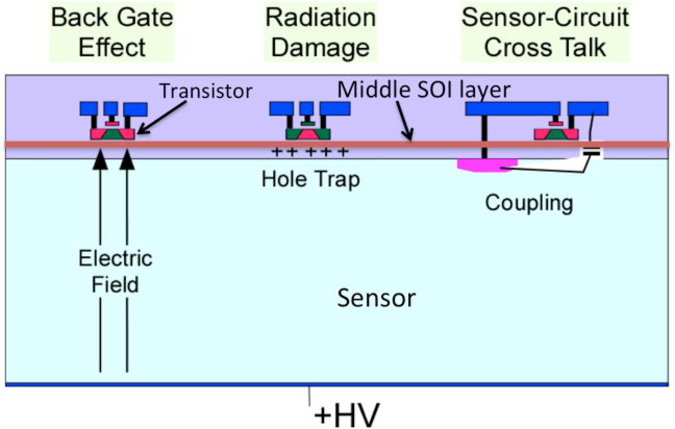
\includegraphics[width=.5\textwidth]{VertexDetector/SOI/SOI_Schematic}
\caption{Major issues in the SOI pixel detector and introduction of a middle-SOI layer}
\label{fig:VertexDetector:SOI:SOI_Schematic}
\end{figure}

\begin{figure}
\centering
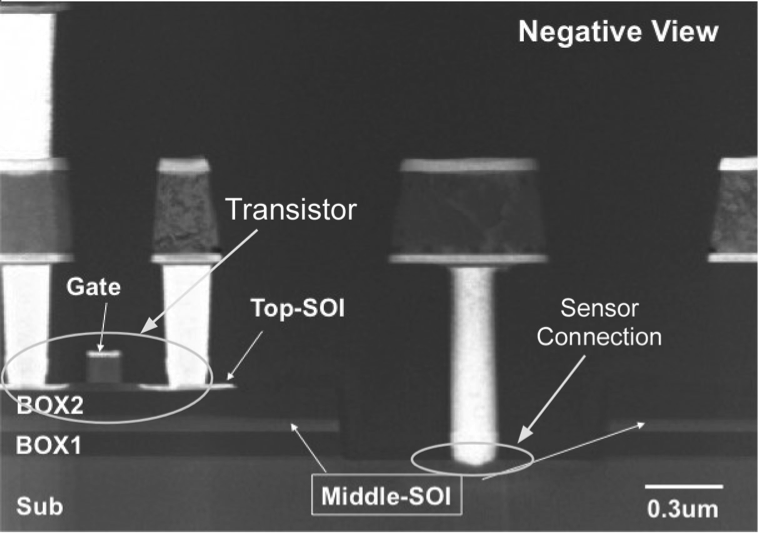
\includegraphics[width=.5\textwidth]{VertexDetector/SOI/crossSectionAfterProcessing}
\caption{Cross section of the double SOI chip after processing}
\label{fig:VertexDetector:SOI:crossSectionAfterProcessing}
\end{figure}

\begin{figure}
\centering
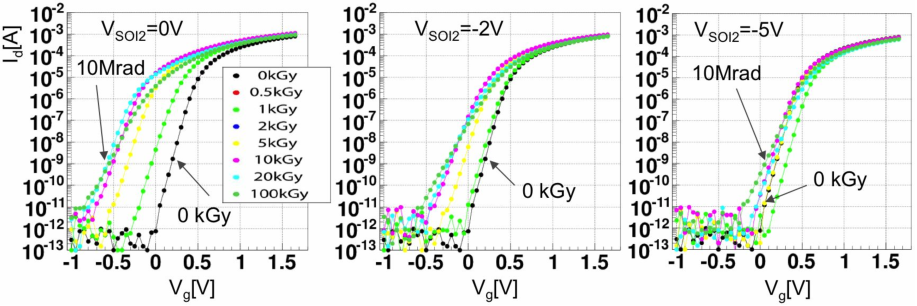
\includegraphics[width=.5\textwidth]{VertexDetector/SOI/thresholdShift}
\caption{Threshold shift recovery by applying compensating voltage (Vsoi2) to the middle Si layer}
\label{fig:VertexDetector:SOI:thresholdShift}
\end{figure}

\subsection{Engineering Challenges}
The impact parameter resolution for the ILC vertex detector is required to be a few \micron. This means the pixel size must be less than about \unit[20]{$\micron^2$}. On the other hand, each pixel must register arrival time of the hits during bunch train, which requires many transistors and capacitors to be located in each pixel.
A solution to this is 3D vertical integration of the circuit layers. SOI technology is ideally suited for 3D integration, since the thinning is stopped at the buried oxide (BOX). We already tried 3D SOI pixel chip in collaboration with T-Micro Co. Ltd. The process flow of micro-bump 3D connection is shown in Figure~\ref{fig:VertexDetector:SOI:microbump3D}. This process achieves a resistance of ($\sim$\unit[6]{$\Omega$}/bump) between upper and lower tiers for 1,000 daisy chain (2,000 bumps) as shown in Figure~\ref{fig:VertexDetector:SOI:resistanceOfDaisyChain}.
However, to achieve the density of digital circuitry necessary for ILC operations, \unit[32]{nm} technology may be necessary for the upper tier in the ILC. This requires bonding of two different technology wafers. The 3D integration of different technology wafers (or chips) is still an engineering challenge.

\begin{figure}
\centering
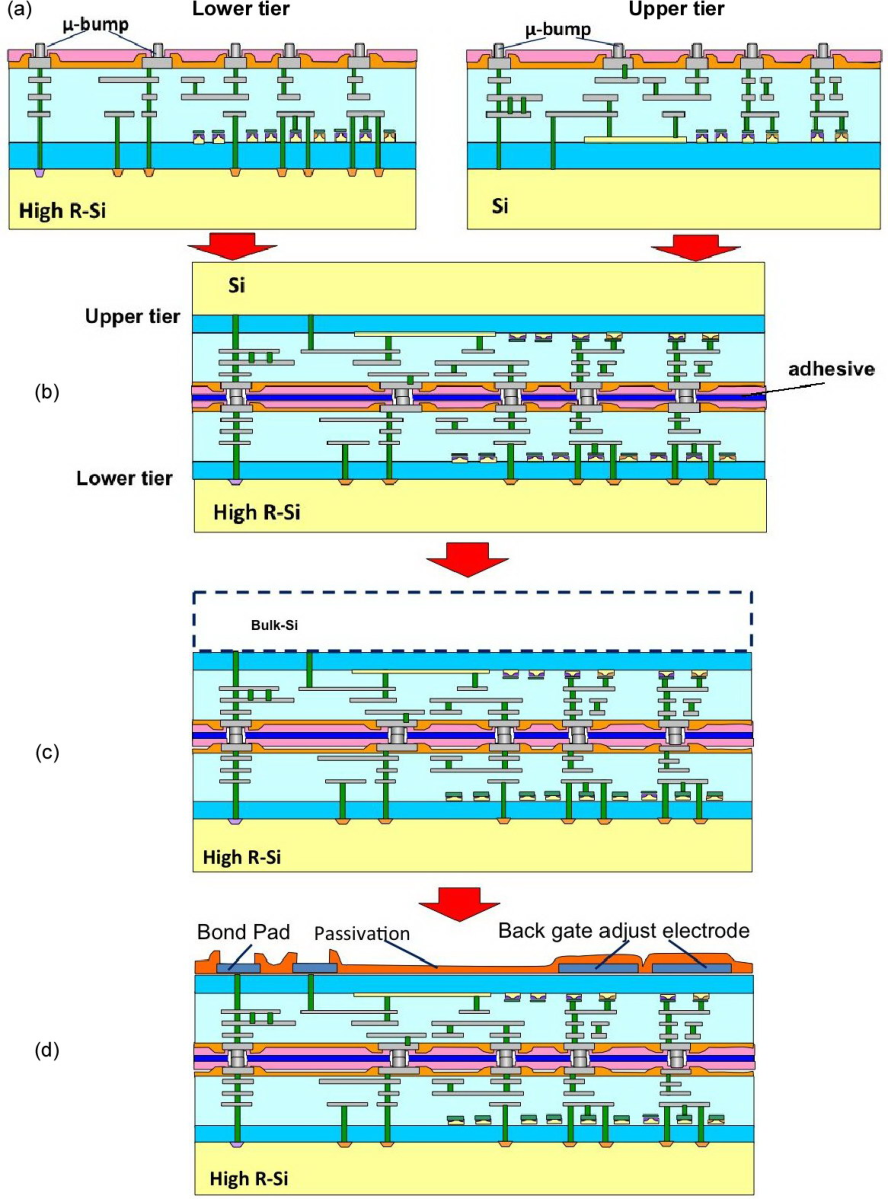
\includegraphics[width=.5\textwidth]{VertexDetector/SOI/microBump3DIntegration}
\caption{Micro-bump 3D integration process flow of the SOI pixel}
\label{fig:VertexDetector:SOI:microbump3D}
\end{figure}

\begin{figure}
\centering
\includegraphics[width=.5\textwidth]{VertexDetector/SOI/resistanceOfDaisyChain}
\caption{Resistance of micro-bump daisy chain between upper and lower tiers}
\label{fig:VertexDetector:SOI:resistanceOfDaisyChain}
\end{figure}

\subsection{Future Plans}
Detector R\&D plans for the coming years;
We are planning following items for the coming year.
\begin{itemize}
\item Sep. 2014 : Complete architecture study for the ILC pixel detector.
\item Mar. 2015 : Design and fabrication of first test chip for the ILC.
\item Dec. 2015 : Beam test of the test chip.
\end{itemize}
